\scanpage{5}

\[\deleted{\begin{array}{ccc}
p_0/p_1&p_{12}\quad p_{23}\quad p_{31}&\delta_1\quad\delta_2\quad\delta_3\\
\delta_0&\deleted{\unsure{\sigma p_{12}\quad\sigma p}}&\\
&p_{21}\quad p_{32}\quad p_{13}&
\end{array}}\]
\mspage{\textcircled{2}}
\[\deleted{\delta_0p_0},\deleted{\delta_0p_1},\quad\mathrm{id},\sigma\]
\diagram{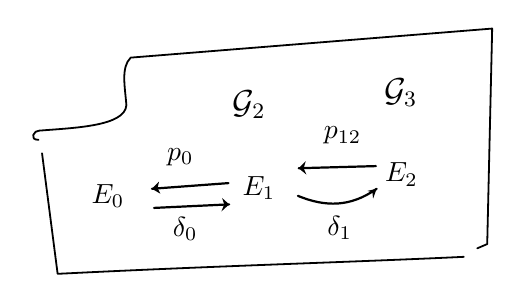
\begin{tikzpicture}[x=.009cm,y=-.009cm,line cap=round,line join=round]
\node at (113,251) {$E_0$};
\node at (326,240) {$E_1$};
\node at (527,221) {$E_2$};
\node at (312,123) {\large$\mathcal G_2$};
\node at (526,105) {\large$\mathcal G_3$};
\draw[line width=.8pt] (283,233) -- (175,241);
\fill (175,241) -- (185,231) -- (183,240) -- (187,248) -- cycle;
\node at (215,196) {$p_0$};
\draw[line width=.8pt] (178,268) -- (284,263);
\fill (284,263) -- (274,254) -- (277,263) -- (273,273) -- cycle;
\node at (222,297) {$\delta_0$};
\draw[line width=.8pt] (491,209) -- (382,212);
\fill (382,212) -- (392,202) -- (389,212) -- (393,221) -- cycle;
\node at (444,166) {$p_{12}$};
\draw[line width=.8pt] (381,251) .. controls (420,267) and (455,267) .. (492,241);
\fill (492,241) -- (479,244) -- (486,246) -- (487,255) -- cycle;
\node at (440,296) {$\delta_1$};
\draw[line width=.65pt] (15,172) .. controls (1,172) and (9,158) .. (16,159)
 .. controls (65,155) and (137,153) .. (139,123)
 .. controls (137,97) and (131,70) .. (145,56)
 -- (655,15) -- (648,319) -- (634,325);
\draw[line width=.65pt] (20,191) -- (42,361)
 .. controls (260,350) and (470,344) .. (615,337);
\end{tikzpicture}}
\[\deleted{\delta_1p_{12}}\]
\[\boxed{\begin{aligned}p_0\delta_0&=\mathrm{id}_{E_0}\\\sigma\delta_0&=\delta_0\end{aligned}}\]
\[\boxed{\begin{aligned}
p_{12}\delta_1&=\sigma\qquad\text{(involution}\\
p_{12}\overset{\deleted{\unsure{\mathrm{id}}}}{\underbrace{\rho\delta_1}_{\delta_3}}&=\delta_0p_0\qquad\text{(idempotent)}\\
p_{12}(\underbrace{\rho^2\delta_1}_{\delta_2})&=\mathrm{id}
\end{aligned}}\]
\margin{$\boxed{\deleted{p_0/p_1}}$\\\diagram{\begin{tikzcd}[execute at end picture={\foreach \ovalnode in {ovalp}{\begingroup\pgfextractx{\dimen0}{\pgfpointdiff{\pgfpointanchor{\ovalnode}{west}}{\pgfpointanchor{\ovalnode}{east}}}\pgfextracty{\dimen2}{\pgfpointdiff{\pgfpointanchor{\ovalnode}{south}}{\pgfpointanchor{\ovalnode}{north}}}\dimen0=.7071067812\dimen0\dimen2=.7071067812\dimen2\draw (\ovalnode.center) ellipse[x radius=\the\dimen0,y radius=\the\dimen2];\endgroup}}]|[alias=ovalp,rectangle,draw=none]|p_0,p_1\end{tikzcd}}}
\diagram{\begin{tikzcd}[ampersand replacement=\&,column sep=large,row sep=small,execute at end picture={\foreach \ovalnode in {ovald,ovaldp,ovalpp}{\begingroup\pgfextractx{\dimen0}{\pgfpointdiff{\pgfpointanchor{\ovalnode}{west}}{\pgfpointanchor{\ovalnode}{east}}}\pgfextracty{\dimen2}{\pgfpointdiff{\pgfpointanchor{\ovalnode}{south}}{\pgfpointanchor{\ovalnode}{north}}}\dimen0=.7071067812\dimen0\dimen2=.7071067812\dimen2\draw (\ovalnode.center) ellipse[x radius=\the\dimen0,y radius=\the\dimen2];\endgroup}}]
\boxed{\begin{gathered}\sigma_1\delta_1=\delta_1\\p_{12}\sigma_3=\underbrace{\sigma p_{12}}_{p_{21}}\end{gathered}}\&|[alias=ovald,rectangle,draw=none]|\delta_1,\delta_2,\delta_3\arrow[l,bend right=15,shorten <=1em]\&|[alias=ovaldp,rectangle,draw=none]|\begin{gathered}\delta'_1=\delta_1\sigma\\\delta'_2=\delta_2\sigma\\\delta'_3=\delta_3\sigma\end{gathered}\\
\&|[alias=ovalpp,rectangle,draw=none]|\begin{gathered}p_{12},p_{23},p_{31},\unsure{{}^3}\\p_{21},p_{32},p_{13}\end{gathered}\&
\end{tikzcd}}
\[\boxed{\begin{gathered}
\rho(\delta_1\delta_0)=\sigma_1(\delta_1\delta_0)=\delta_1\delta_0\\
\text{i.e.}\qquad g(\delta_1\delta_0)=\delta_1\delta_0\quad\text{pour }g\in\mathcal G_3
\end{gathered}}\]
\[\boxed{p_0p_{12}\sigma_1=\underbrace{p_0p_{12}}_{\unsure{q_1|p_1}}}\]
\margin{\diagram{\begin{tikzcd}[execute at end picture={\foreach \ovalnode in {ovalq}{\begingroup\pgfextractx{\dimen0}{\pgfpointdiff{\pgfpointanchor{\ovalnode}{west}}{\pgfpointanchor{\ovalnode}{east}}}\pgfextracty{\dimen2}{\pgfpointdiff{\pgfpointanchor{\ovalnode}{south}}{\pgfpointanchor{\ovalnode}{north}}}\dimen0=.7071067812\dimen0\dimen2=.7071067812\dimen2\draw (\ovalnode.center) ellipse[x radius=\the\dimen0,y radius=\the\dimen2];\endgroup}}]|[alias=ovalq,rectangle,draw=none]|q_1,q_2,q_3\end{tikzcd}}}
\margin{4}

